\documentclass[../main.tex]{subfiles}

\begin{document}

\chapter{Roundoff and Truncation Errors}
\label{chap:chap_4}

\begin{center}
\Large{\textbf{CHAPTER OBJECTIVES}}    
\end{center}
The primary objective of this chapter is to acquaint you with the major sources of
errors involved in numerical methods. Specific objectives and topics covered are
\begin{itemize}
\item Understanding the distinction between accuracy and precision.
\item Learning how to quantify error.
\item Learning how error estimates can be used to decide when to terminate an iterative
calculation.
\item Understanding how roundoff errors occur because digital computers have a
limited ability to represent numbers.
\item Understanding why floating-point numbers have limits on their range and
precision.
\item Recognizing that truncation errors occur when exact mathematical formulations
are represented by approximations.
\item Knowing how to use the Taylor series to estimate truncation errors.
\item Understanding how to write forward, backward, and centered finite-difference
approximations of first and second derivatives.
\item Recognizing that efforts to minimize truncation errors can sometimes increase
roundoff errors.
\end{itemize}

\bigskip
\noindent
\Large{YOU'VE GOT A PROBLEM}
\bigskip

\noindent
\normalsize{In Chap. 1 you developed a numerical model for the velocity of a bungee jumper. To
solve the problem with a computer, you had to approximate the derivative of velocity
with a finite difference.}

\bigskip
$\dfrac{dv}{dt}\cong\dfrac{\mid\Delta v}{\Delta t}=
\dfrac{v(t_{i+1})-v(t_i)}{t_{i+1}-t_i}$

\bigskip
\noindent
Thus, the resulting solution is not exact --- that is, it has error.

In addition, the computer you use to obtain the solution is also an imperfect tool. Because
it is a digital device, the computer is limited in its ability to represent the magnitudes
and precision of numbers. Consequently, the machine itself yields results that contain error.

So both your mathematical approximation and your digital computer cause your resulting
model prediction to be uncertain. Your problem is: How do you deal with such uncertainty?
In particular, is it possible to understand, quantify and control such errors in
order to obtain acceptable results? This chapter introduces you to some approaches and
concepts that engineers and scientists use to deal with this dilemma.

\bigskip
\section[ERRORS]{ERRORS}

Engineers and scientists constantly find themselves having to accomplish objectives based
on uncertain information. Although perfection is a laudable goal, it is rarely if ever attained.
For example, despite the fact that the model developed from Newton's second law
is an excellent approximation, it would never in practice exactly predict the jumper's fall.
A variety of factors such as winds and slight variations in air resistance would result in deviations
from the prediction. If these deviations are systematically high or low, then we
might need to develop a new model. However, if they are randomly distributed and tightly
grouped around the prediction, then the deviations might be considered negligible and the
model deemed adequate. Numerical approximations also introduce similar discrepancies
into the analysis.

This chapter covers basic topics related to the identification, quantification, and minimization
of these errors. General information concerned with the quantification of error is
reviewed in this section. This is followed by Sections 4.2 and 4.3, dealing with the two
major forms of numerical error: roundoff error (due to computer approximations) and truncation
error (due to mathematical approximations). We also describe how strategies to reduce
truncation error sometimes increase roundoff. Finally, we briefly discuss errors not
directly connected with the numerical methods themselves. These include blunders, model
errors, and data uncertainty.

\subsection{Accuracy and Precision}
\noindent
The errors associated with both calculations and measurements can be characterized with
regard to their accuracy and precision. Accuracy refers to how closely a computed or measured
value agrees with the true value. Precision refers to how closely individual computed
or measured values agree with each other.

These concepts can be illustrated graphically using an analogy from target practice.
The bullet holes on each target in Fig. 4.1 can be thought of as the predictions of a numerical
technique, whereas the bull's-eye represents the truth. Inaccuracy (also called bias) is
defined as systematic deviation from the truth. Thus, although the shots in Fig. 4.1c are
more tightly grouped than in Fig. 4.1a, the two cases are equally biased because they are
both centered on the upper left quadrant of the target. Imprecision (also called uncertainty),
on the other hand, refers to the magnitude of the scatter. Therefore, although Fig. 4.1b and
d are equally accurate (i.e., centered on the bull's-eye), the latter is more precise because
the shots are tightly grouped.

\begin{figure}[h]
    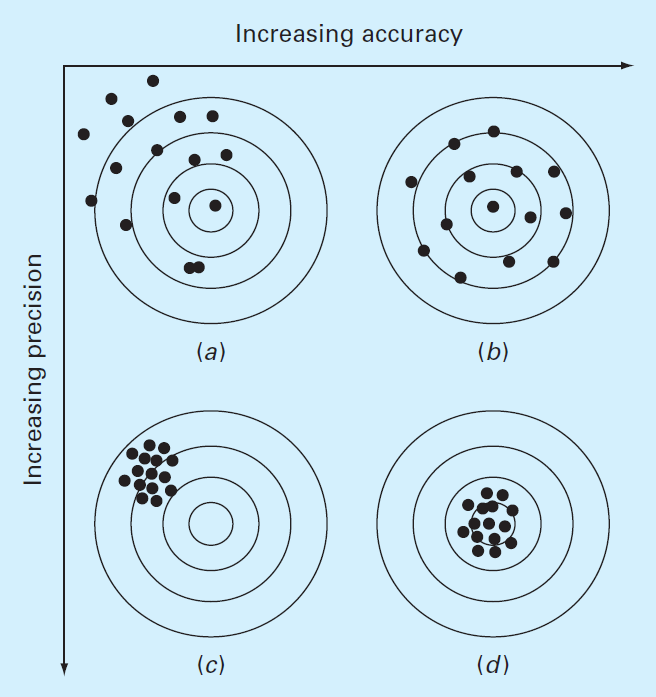
\includegraphics[width=0.55\linewidth]{./images/fig_4_1.png}    
    \caption{An example from marksmanship illustrating the concepts of accuracy and precision:
    (\emph{a}) inaccurate and imprecise, (\emph{b}) accurate and imprecise, (\emph{c}) inaccurate and precise,
    and (\emph{d}) accurate and precise.}
\end{figure}

\bigskip
Numerical methods should be sufficiently accurate or unbiased to meet the requirements
of a particular problem. They also should be precise enough for adequate design.
In this book, we will use the collective term \emph{error} to represent both the inaccuracy and
imprecision of our predictions.

\subsection{Error Definitions}
\noindent
Numerical errors arise from the use of approximations to represent exact mathematical operations
and quantities. For such errors, the relationship between the exact, or true, result
and the approximation can be formulated as
\newline

True value = approximation + error
\hfill
(4.1)
\newline

\noindent
By rearranging Eq. (4.1), we find that the numerical error is equal to the discrepancy
between the truth and the approximation, as in
\newline

$E_t$ = true value - approximation
\hfill
(4.2)
\newline

\noindent
where $E_t$ is used to designate the exact value of the error. The subscript t is included to designate
that this is the ``true'' error. This is in contrast to other cases, as described shortly,
where an ``approximate'' estimate of the error must be employed. Note that the true error is
commonly expressed as an absolute value and referred to as the \emph{absolute error}.

A shortcoming of this definition is that it takes no account of the order of magnitude of
the value under examination. For example, an error of a centimeter is much more significant if we are measuring a rivet than a bridge. One way to account for the magnitudes of the
quantities being evaluated is to normalize the error to the true value, as in$\mid$
\newline

True fractional relative error = $\dfrac{\text{true value -- approximation}}{\text{true value}}$
\newline

\noindent
The relative error can also be multiplied by 100\% to express it as
\newline

$\epsilon_t = \dfrac{\text{true value -- approximation}}{true value} 100\%$
\hfill
(4.3)
\newline

\noindent
where $\epsilon_t$ designates the true percent relative error.

For example, suppose that you have the task of measuring the lengths of a bridge and
a rivet and come up with 9999 and 9 cm, respectively. If the true values are 10,000 and
10 cm, respectively, the error in both cases is 1 cm. However, their percent relative errors
can be computed using Eq. (4.3) as 0.01\% and 10\%, respectively. Thus, although both measurements
have an absolute error of 1 cm, the relative error for the rivet is much greater. We
would probably conclude that we have done an adequate job of measuring the bridge,
whereas our estimate for the rivet leaves something to be desired.

Notice that for Eqs. (4.2) and (4.3), $E$ and $\epsilon$ are subscripted with a \emph{t} to signify that the
error is based on the true value. For the example of the rivet and the bridge, we were provided
with this value. However, in actual situations such information is rarely available.
For numerical methods, the true value will only be known when we deal with functions that
can be solved analytically. Such will typically be the case when we investigate the theoretical
behavior of a particular technique for simple systems. However, in real-world applications,
we will obviously not know the true answer \emph{a priori}. For these situations, an
alternative is to normalize the error using the best available estimate of the true value --- that
is, to the approximation itself, as in
\newline

$\epsilon_a = \dfrac{\text{approximate error}}{\text{approximation}}100\%$
\hfill
(4.4)
\newline

\noindent
where the subscript a signifies that the error is normalized to an approximate value. Note
also that for real-world applications, Eq. (4.2) cannot be used to calculate the error term in
the numerator of Eq. (4.4). One of the challenges of numerical methods is to determine
error estimates in the absence of knowledge regarding the true value. For example, certain
numerical methods use \emph{iteration} to compute answers. In such cases, a present approximation
is made on the basis of a previous approximation. This process is performed repeatedly,
or iteratively, to successively compute (hopefully) better and better approximations.
For such cases, the error is often estimated as the difference between the previous and present
approximations. Thus, percent relative error is determined according to
\newline

$\epsilon_a = \dfrac{\text{present approximation -- previous approximation}}
{\text{present approximation}}100\%$
\hfill
(4.5)
\newline

\noindent
This and other approaches for expressing errors is elaborated on in subsequent chapters.

The signs of Eqs. (4.2) through (4.5) may be either positive or negative. If the approximation
is greater than the true value (or the previous approximation is greater than the current
approximation), the error is negative; if the approximation is less than the true value,
the error is positive. Also, for Eqs. (4.3) to (4.5), the denominator may be less than zero,
which can also lead to a negative error. Often, when performing computations, we may not
be concerned with the sign of the error but are interested in whether the absolute value of the
percent relative error is lower than a prespecified tolerance $\epsilon_s$. Therefore, it is often useful
to employ the absolute value of Eq. (4.5). For such cases, the computation is repeated until
\newline

$\left\lvert\epsilon_a\right\rvert < \epsilon_s$
\hfill
(4.6)
\newline

\noindent
This relationship is referred to as a \emph{stopping criterion}. If it is satisfied, our result is assumed
to be within the prespecified acceptable level $\epsilon_s$ . Note that for the remainder of this text, we
almost always employ absolute values when using relative errors.

It is also convenient to relate these errors to the number of significant figures in the approximation.
It can be shown (Scarborough, 1966) that if the following criterion is met, we
can be assured that the result is correct to \emph{at least n} significant figures.
\newline

$\epsilon_s = (0.5 \times 10^{2-n})\%$
\hfill
(4.7)
\newpage

\begin{example} Error Estimates for Iterative Methods
    \bigskip
    \newline
    \textbf{Problem Statement.}\quad In mathematics, functions can often be represented by infinite series.
    For example, the exponential function can be computed using
    \newline
    
    $e^x = 1+x+\dfrac{x^2}{2}+\dfrac{x^3}{3!}+\hdots+\dfrac{x^n}{n!}$
    \hfill (E4.11)
    \newline

    \noindent
    Thus, as more terms are added in sequence, the approximation becomes a better and better
    estimate of the true value of $e^x$. Equation (E4.1.1) is called a \emph{Maclaurin series expansion}.

    Starting with the simplest version, $e^x = 1$, add terms one at a time in order to estimate
    $e^{0.5}$. After each new term is added, compute the true and approximate percent relative errors
    with Eqs. (4.3) and (4.5), respectively. Note that the true value is $e^{0.5} = 1.648721\dots$ Add
    terms until the absolute value of the approximate error estimate $\epsilon_a$ falls below a prespecified
    error criterion $\epsilon_s$ conforming to three significant figures.
    \newline

    \noindent
    \textbf{Solution.}\quad First, Eq. (4.7) can be employed to determine the error criterion that ensures a
    result that is correct to at least three significant figures:
    \newline

    $\epsilon_s = (0.5\times10^{2-3})\%=0.05\%$
    \newline

    \noindent
    Thus, we will add terms to the series until $\epsilon_a$ falls below this level.
    
    The first estimate is simply equal to Eq. (E4.1.1) with a single term. Thus, the first
    estimate is equal to 1. The second estimate is then generated by adding the second term
    as in
    \newline

    $e^x=1+x$
    \newline

    \noindent
    or for $x=0.5$
    \newline

    $e^{0.5}=1+0.5 = 1.5$
    \newline

    \noindent
    This represents a true percent relative error of [Eq. (4.3)]
    \newline

    $\epsilon_t = \left\lvert\dfrac{1.648721-1.5}{1.648721}\right\rvert\times100\%=9.02\%$
    \newline

    \noindent
    Equation (4.5) can be used to determine an approximate estimate of the error, as in
    \newline

    $\epsilon_a = \left\lvert\dfrac{1.5-1}{1.5}\times100\%=33.3\% \right\rvert $
    \newline

    \noindent
    Because ${\epsilon_a}$ is not less than the required value of $\epsilon_s$, we would continue the computation by
    adding another term, $x^2/2!$, and repeating the error calculations. The process is continued
    until $\left\lvert\epsilon_a \right\rvert < \epsilon_s$. The entire computation can be summarized as
    \newline

    \begin{figure}[h]
        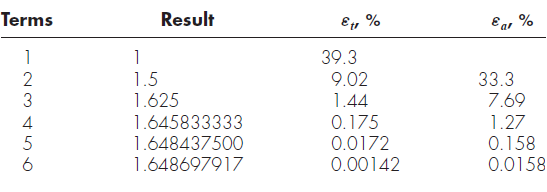
\includegraphics{./images/fig_4_1_1}
    \end{figure}

    \noindent
    Thus, after six terms are included, the approximate error falls below $\epsilon_s=0.05\%$, and the
    computation is terminated. However, notice that, rather than three significant figures, the
    result is accurate to five! This is because, for this case, both Eqs. (4.5) and (4.7) are conservative.
    That is, they ensure that the result is at least as good as they specify. Although,
    this is not always the case for Eq. (4.5), it is true most of the time.
\end{example}
\newpage

\subsection{Computer Algorithm for Iterative Calculations}

\noindent
Many of the numerical methods described in the remainder of this text involve iterative
calculations of the sort illustrated in Example 4.1. These all entail solving a mathematical
problem by computing successive approximations to the solution starting from an initial
guess.

The computer implementation of such iterative solutions involves loops. As we saw in
Sec. 3.3.2, these come in two basic flavors: count-controlled and decision loops. Most iterative
solutions use decision loops. Thus, rather than employing a pre-specified number of
iterations, the process typically is repeated until an approximate error estimate falls below
a stopping criterion as in Example 4.1.

To do this for the same problem as Example 4.1, the series expansion can be expressed
as
\newline

$e^x\cong \mathlarger{\sum}_{i=0}^{n}\dfrac{x^n}{n!}$
\newline

\noindent
An M-file to implement this formula is shown in Fig. 4.2. The function is passed the value
to be evaluated (x) along with a stopping error criterion (es) and a maximum allowable
number of iterations (maxit). If the user omits either of the latter two parameters, the function
assigns default values.
\newline

\begin{figure}[h]
    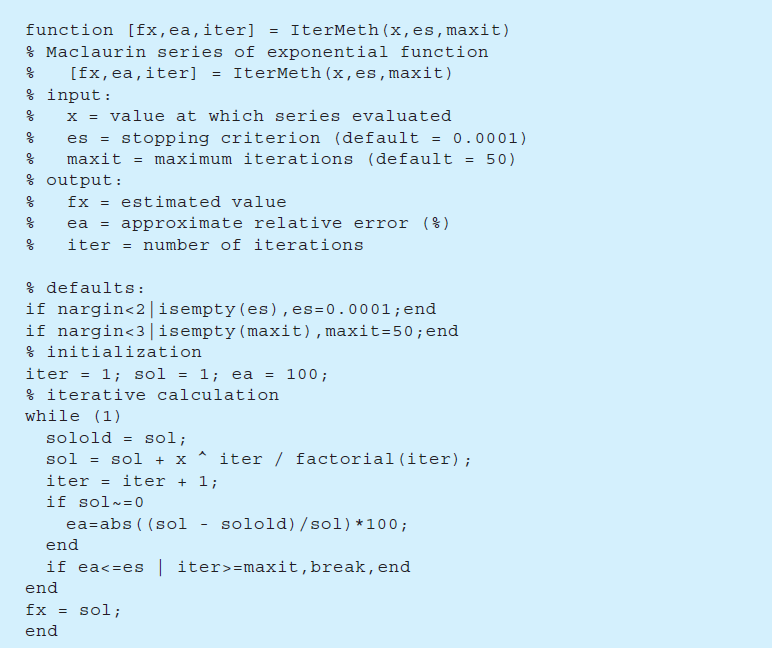
\includegraphics{./images/fig_4_2}
    \caption{An M-file to solve an iterative calculation. This example is set up to evaluate the Maclaurin series
    expansion for ex as described in Example 4.1.}
\end{figure}

The function then initializes three variables: \emph{(a)} \texttt{iter}, which keeps track of the number
of iterations, \emph{(b)} \texttt{sol}, which holds the current estimate of the solution, and \emph{(c)} a variable,
\texttt{ea}, which holds the approximate percent relative error. Note that \emph{ea} is initially set to a value
of 100 to ensure that the loop executes at least once.

These initializations are followed by a decision loop that actually implements the
iterative calculation. Prior to generating a new solution, the previous value, \texttt{sol}, is first assigned
to \texttt{solold}. Then a new value of \texttt{sol} is computed and the iteration counter is incremented.
If the new value of \texttt{sol} is nonzero, the percent relative error, \texttt{ea}, is determined.
The stopping criteria are then tested. If both are false, the loop repeats. If either is
true, the loop terminates and the final solution is sent back to the function call.

When the M-file is implemented, it generates an estimate for the exponential function
which is returned along with the approximate error and the number of iterations. For
example, $e^1$ can be evaluated as

\texttt{>> format long}

\texttt{>> [approxval, ea, iter] = IterMeth(1,1e-6,100)}

\texttt{approxval = 2.718281826198493}

\texttt{ea = 9.216155641522974e-007}

\texttt{iter =12}\\

We can see that after 12 iterations, we obtain a result of 2.7182818 with an
approximate error estimate of $= 9.2162 \times 10^{-7}\%$. The result can be verified by using
the built-in \texttt{exp} function to directly calculate the exact value and the true percent relative
error,\\

\texttt{>> trueval=exp(1)}

\texttt{trueval =2.718281828459046}

\texttt{>> et=abs((trueval- approxval)/trueval)*100}

\texttt{et =8.316108397236229e-008}\\
    
\noindent
As was the case with Example 4.1, we obtain the desirable outcome that the true error is
less than the approximate error.
\vspace{10 mm}

\section{ROUNDOFF ERRORS}
\emph{Roundoff errors} arise because digital computers cannot represent some quantities exactly.
They are important to engineering and scientific problem solving because they
can lead to erroneous results. In certain cases, they can actually lead to a calculation
going unstable and yielding obviously erroneous results. Such calculations are said to
be \emph{ill-conditioned}. Worse still, they can lead to subtler discrepancies that are difficult
to detect.

There are two major facets of roundoff errors involved in numerical calculations:

\begin{enumerate}
    \item Digital computers have magnitude and precision limits on their ability to represent
    numbers.
    \item Certain numerical manipulations are highly sensitive to roundoff errors. This can result
    from both mathematical considerations as well as from the way in which computers
    perform arithmetic operations.
\end{enumerate}

\subsection{Computer Number Representation}
Numerical roundoff errors are directly related to the manner in which numbers are stored
in a computer. The fundamental unit whereby information is represented is called a \emph{word}.
This is an entity that consists of a string of binary \emph{digits}, or \emph{bits}. Numbers are typically
stored in one or more words. To understand how this is accomplished, we must first review
some material related to number systems.

A \emph{number system} is merely a convention for representing quantities. Because we have
10 fingers and 10 toes, the number system that we are most familiar with is the \emph{decimal}, or
\emph{base-10}, number system. A base is the number used as the reference for constructing the
system. The base-10 system uses the 10 digits---0, 1, 2, 3, 4, 5, 6, 7, 8, and 9---to represent
numbers. By themselves, these digits are satisfactory for counting from 0 to 9.

For larger quantities, combinations of these basic digits are used, with the position or
\emph{place value} specifying the magnitude. The rightmost digit in a whole number represents a
number from 0 to 9. The second digit from the right represents a multiple of 10. The third
digit from the right represents a multiple of 100 and so on. For example, if we have the
number 8642.9, then we have eight groups of 1000, six groups of 100, four groups of 10,
two groups of 1, and nine groups of 0.1, or\\

$(8 \times 10^3) + (6 \times 10^2) + (4 \times 10^1) + (2 \times 10^0) + (9 \times 10^{−1}) = 8642.9$\\

\noindent
This type of representation is called \emph{positional notation}.

Now, because the decimal system is so familiar, it is not commonly realized that
there are alternatives. For example, if human beings happened to have eight fingers and
toes we would undoubtedly have developed an \emph{octal}, or \emph{base-8}, representation. In the
same sense, our friend the computer is like a two-fingered animal who is limited to two
states---either 0 or 1. This relates to the fact that the primary logic units of digital computers
are on/off electronic components. Hence, numbers on the computer are represented
with a \emph{binary}, or \emph{base-2}, system. Just as with the decimal system, quantities
can be represented using positional notation. For example, the binary number 101.1 is
equivalent to $(1 \times 2^2)+(0 \times 2^1) + (1 \times 2^0) + (1 \times 2^{−1}) = 4 + 0 + 1 + 0.5 = 5.5$ in the
decimal system.
\newpage

\noindent
\textbf{Integer Representation.}\quad
Now that we have reviewed how base-10 numbers can be represented
in binary form, it is simple to conceive of how integers are represented on a computer.
The most straightforward approach, called the \emph{signed magnitude method}, employs
the first bit of a word to indicate the sign, with a 0 for positive and a 1 for negative. The remaining
bits are used to store the number. For example, the integer value of 173 is represented
in binary as 10101101:\\

$(10101101)_2= 2^7 + 2^5 + 2^3 + 2^2 + 2^0 = 128 + 32 + 8 + 4 + 1 = (173)_{10}$\\

\noindent
Therefore, the binary equivalent of --173 would be stored on a 16-bit computer, as depicted
in Fig. 4.3.

If such a scheme is employed, there clearly is a limited range of integers that can be represented.
Again assuming a 16-bit word size, if one bit is used for the sign, the 15 remaining
bits can represent binary integers from 0 to 111111111111111. The upper limit can be converted
to a decimal integer, as in 

$(1 \times2^{14}) +(1 \times2^{13}) +\hdots +(1 \times2^{1}) +(1 \times2^{0}) = 32,767$.\\


\begin{figure}[h]
    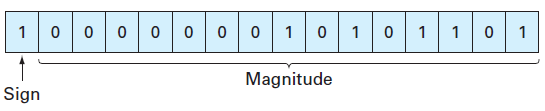
\includegraphics{./images/fig_4_3}
    \caption{The binary representation of the decimal integer –173 on a 16-bit computer using the signed
    magnitude method.}
\end{figure}

\noindent
Note that this value can be simply evaluated as $2^{15}-1$. Thus, a 16-bit computer word can
store decimal integers ranging from --32,767 to 32,767.

In addition, because zero is already defined as 0000000000000000, it is redundant
to use the number 1000000000000000 to define a ``minus zero''. Therefore, it is conventionally
employed to represent an additional negative number: --32,768, and the range is
from --32,768 to 32,767. For an n-bit word, the range would be from  $-2^{n-1}$ to $2^{n-1}-1$.
Thus, 32-bit integers would range from --2,147,483,648 to +2,147,483,647.

Note that, although it provides a nice way to illustrate our point, the signed magnitude
method is not actually used to represent integers for conventional computers. A preferred
approach called the 2s \emph{complement} technique directly incorporates the sign into the
number's magnitude rather than providing a separate bit to represent plus or minus.
Regardless, the range of numbers is still the same as for the signed magnitude method
described above.

The foregoing serves to illustrate how all digital computers are limited in their capability
to represent integers. That is, numbers above or below the range cannot be represented. A
more serious limitation is encountered in the storage and manipulation of fractional quantities
as described next.\\

\noindent
\textbf{Floating-Point Representation.}\quad Fractional quantities are typically represented in computers
using \emph{floating-point format}. In this approach, which is very much like scientific
notation, the number is expressed as\\

$\pm s\times b^e$\\

\noindent
where s = the \emph{significand} (or \emph{mantissa}), b = the base of the number system being used, and
e = the exponent.

Prior to being expressed in this form, the number is \emph{normalize}d by moving the decimal
place over so that only one significant digit is to the left of the decimal point. This is done so
computer memory is not wasted on storing useless nonsignificant zeros. For example, a value
like 0.005678 could be represented in a wasteful manner as 0.005678 × 100. However, normalization
would yield $5.678 \times 10^{-3}$ which eliminates the useless zeroes.

Before describing the base-2 implementation used on computers, we will first explore
the fundamental implications of such floating-point representation. In particular,
what are the ramifications of the fact that in order to be stored in the computer, both
the mantissa and the exponent must be limited to a finite number of bits? As in the
next example, a nice way to do this is within the context of our more familiar base-10
decimal world.\\

\begin{example} Implications of Floating-Point Representation
    \bigskip
    \newline
    \textbf{Problem Statement.}\quad Suppose that we had a hypothetical base-10 computer with a 5-digit
    word size. Assume that one digit is used for the sign, two for the exponent, and two for the
    mantissa. For simplicity, assume that one of the exponent digits is used for its sign, leaving
    a single digit for its magnitude.\\

    \noindent
    \textbf{Solution.}\quad A general representation of the number following normalization would be\\

    $s_1 d_1 d_2 \times 10^{s_0 d_0}$
    \newpage

    \noindent
    where $s_0$ and $s_1$ = the signs, $d_0$ = the magnitude of the exponent, and $d_1$ and $d_2$ = the magnitude
    of the significand digits.

    Now, let's play with this system. First, what is the largest possible positive quantity
    that can be represented? Clearly, it would correspond to both signs being positive and all
    magnitude digits set to the largest possible value in base-10, that is, 9:\\

    Largest value = $+9.9\times10^{+9}$\\

    \noindent
    So the largest possible number would be a little less than 10 billion. Although this might
    seem like a big number, it's really not that big. For example, this computer would be incapable
    of representing a commonly used constant like Avogadro's number $(6.022 \times 1023)$.
    In the same sense, the smallest possible positive number would be\\

    Smallest value = $+1.0 \times 10^{-9}$\\

    \noindent
    Again, although this value might seem pretty small, you could not use it to represent a
    quantity like Planck's constant $(6.626 \times 10^{-34} J \cdot s)$.
    
    Similar negative values could also be developed. The resulting ranges are displayed in
    Fig. 4.4. Large positive and negative numbers that fall outside the range would cause an
    overflow error. In a similar sense, for very small quantities there is a ``hole'' at zero, and
    very small quantities would usually be converted to zero.
    
    Recognize that the exponent overwhelmingly determines these range limitations. For
    example, if we increase the mantissa by one digit, the maximum value increases slightly to
    $9.99\times 10^9$. In contrast, a one-digit increase in the exponent raises the maximum by 90 orders
    of magnitude to $9.9\times 10^{99}$!
    
    When it comes to precision, however, the situation is reversed. Whereas the significand
    plays a minor role in defining the range, it has a profound effect on specifying the precision.
    This is dramatically illustrated for this example where we have limited the significand to
    only 2 digits. As in Fig. 4.5, just as there is a ``hole'' at zero, there are also ``holes'' between
    values.
    
    For example, a simple rational number with a finite number of digits like $2^{-5} = 0.03125$
    would have to be stored as $3.1 \times 10{−2}$ or 0.031. Thus, a \emph{roundoff error} is introduced. For this
    case, it represents a relative error of\\

    $\dfrac{0.03125-0.031}{0.03125}=0.008$\\

    \begin{figure}[h]
        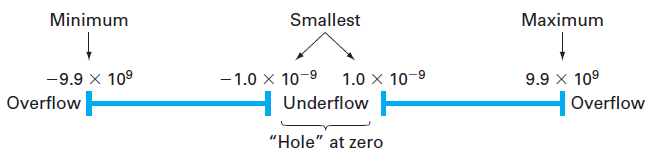
\includegraphics{./images/fig_4_4}
        \caption{The number line showing the possible ranges corresponding to the hypothetical base-10
        floating-point scheme described in Example 4.2.}
    \end{figure}

    \begin{figure}[h]
        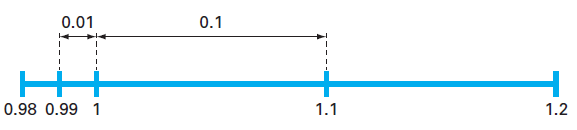
\includegraphics{./images/fig_4_5}
        \caption{A small portion of the number line corresponding to the hypothetical base-10 floating-point
        scheme described in Example 4.2. The numbers indicate values that can be represented
        exactly. All other quantities falling in the ``holes'' between these values would exhibit some
        roundoff error.}
    \end{figure}

    While we could store a number like 0.03125 exactly by expanding the digits of the
    significand, quantities with infinite digits must always be approximated. For example, a
    commonly used constant such as $\pi (=3.14159\hdots)$ would have to be represented as $3.1\times 10^0$
    or 3.1. For this case, the relative error is\\

    $\dfrac{3.14159-3.1}{3.14159} = 0.0132$
    \newpage

    \noindent
    Although adding significand digits can improve the approximation, such quantities will
    always have some roundoff error when stored in a computer.
    
    Another more subtle effect of floating-point representation is illustrated by Fig. 4.5.
    Notice how the interval between numbers increases as we move between orders of magnitude.
    For numbers with an exponent of --1 (i.e., between 0.1 and 1), the spacing is 0.01.
    Once we cross over into the range from 1 to 10, the spacing increases to 0.1. This means
    that the roundoff error of a number will be proportional to its magnitude. In addition, it
    means that the relative error will have an upper bound. For this example, the maximum
    relative error would be 0.05. This value is called the \emph{machine epsilon} (or machine
    precision).\\
\end{example}

As illustrated in Example 4.2, the fact that both the exponent and significand are finite
means that there are both range and precision limits on floating-point representation. Now,
let us examine how floating-point quantities are actually represented in a real computer
using base-2 or binary numbers.

First, let's look at normalization. Since binary numbers consist exclusively of 0s and
1s, a bonus occurs when they are normalized. That is, the bit to the left of the binary point
will always be one! This means that this leading bit does not have to be stored. Hence,
nonzero binary floating-point numbers can be expressed as\\

$\pm (1+f)\times 2^e$\\

\noindent
where f = the \emph{mantissa} (i.e., the fractional part of the significand). For example, if we normalized
the binary number 1101.1, the result would be $1.1011\times (2)^{-3}$ or $(1+0.1011)\times2^{-3}$.

\begin{figure}[h]
    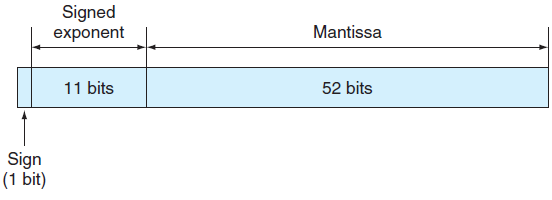
\includegraphics{./images/fig_4_6}
    \caption{The manner in which a floating-point number is stored in an 8-byte word in IEEE doubleprecision
    format.}
\end{figure}

\noindent
Thus, although the original number has five significant bits, we only have to store the four
fractional bits: 0.1011.

By default, MATLAB has adopted the \emph{IEEE double-precision format} in which eight
bytes (64 bits) are used to represent floating-point numbers. As in Fig. 4.6, one bit is reserved
for the number's sign. In a similar spirit to the way in which integers are stored, the
exponent and its sign are stored in 11 bits. Finally, 52 bits are set aside for the mantissa.
However, because of normalization, 53 bits can be stored.

Now, just as in Example 4.2, this means that the numbers will have a limited range and
precision. However, because the IEEE format uses many more bits, the resulting number
system can be used for practical purposes.\\

\noindent
\textbf{Range}\quad In a fashion similar to the way in which integers are stored, the 11 bits used for
the exponent translates into a range from --1022 to 1023. The largest positive number can
be represented in binary as\\

Largest value = $+1.1111\hdots1111\times 2^{+1023}$\\

\noindent
where the 52 bits in the mantissa are all 1. Since the significant is approximately 2 (it is
actually $2-2^{-52}$), the largest value is therefore $2^{1024}=1.7977\times 10^{308}$. In a similar
fashion, the smallest positive number can be represented as\\

Smallest value = $+1.0000\hdots 0000\times 2^{-1022}$\\

\noindent
This value can be translated into a base-10 value of $2^{-1022}=2.2251\times10^{-308}$

\noindent
\textbf{Precision.}\quad The 52 bits used for the mantissa correspond to about 15 to 16 base-10 digits.
Thus, $\pi$ would be expressed as

\texttt{>> format long}

\texttt{>> $\pi$}

\texttt{ans = 3.14159265358979}
\newpage

\noindent
Note that the machine epsilon is $2^{-52}=2.2204\times 10^{-16}$\\

MATLAB has a number of built-in functions related to its internal number representation.
For example, the \texttt{realmax} function displays the largest positive real number:

\texttt{>> format long}

\texttt{>> realmax}

\texttt{ans = 1.797693134862316e+308}\\

Numbers occurring in computations that exceed this value create an overflow. InMATLAB
they are set to infinity, \texttt{inf}. The \texttt{realmin} function displays the smallest positive real
number:

\texttt{>> realmin}

\texttt{ans = 2.225073858507201e-308}\\

\noindent
Numbers that are smaller than this value create an \emph{underflow} and, in MATLAB, are set to
zero. Finally, the \texttt{eps} function displays the machine epsilon:\\

\subsection{Arithmetic Manipulations of Computer Numbers}

\noindent
Aside from the limitations of a computer's number system, the actual arithmetic manipulations
involving these numbers can also result in roundoff error. To understand how this
occurs, let's look at how the computer performs simple addition and subtraction.

Because of their familiarity, normalized base-10 numbers will be employed to illustrate
the effect of roundoff errors on simple addition and subtraction. Other number bases
would behave in a similar fashion. To simplify the discussion, we will employ a hypothetical
decimal computer with a 4-digit mantissa and a 1-digit exponent.

When two floating-point numbers are added, the numbers are first expressed so that
they have the same exponents. For example, if we want to add $1.557 + 0.04341$, the computer
would express the numbers as \\$0.1557\times 10^1 + 0.004341\times 10^1$. Then the mantissas
are added to give $0.160041 \times 101$. Now, because this hypothetical computer only carries a
4-digit mantissa, the excess number of digits get chopped off and the result is $0.1600\times 101$.
Notice how the last two digits of the second number (41) that were shifted to the right have
essentially been lost from the computation.

Subtraction is performed identically to addition except that the sign of the subtrahend
is reversed. For example, suppose that we are subtracting 26.86 from 36.41. That is,\\

\begin{tabular}{c c c}
        & $0.3641 \times 10^2$\\
    -   & $0.2686 \times 10^2$\\
        \hline
        & $0.0955 \times 10^2$\\
\end{tabular}\\

For this case the result must be normalized because the leading zero is unnecessary. So
we must shift the decimal one place to the right to give $0.9550 \times 10^1 = 9.550$. Notice that
the zero added to the end of the mantissa is not significant but is merely appended to fill the
empty space created by the shift. Even more dramatic results would be obtained when the
numbers are very close as in\\

\begin{tabular}{c c c}
    & $0.7642 \times 10^3$\\
-   & $0.7641 \times 10^3$\\
    \hline
    & $0.0001 \times 10^3$\\
\end{tabular}\\

\noindent
which would be converted to $0.1000 \times 100 = 0.1000$. Thus, for this case, three nonsignificant
zeros are appended.
The subtracting of two nearly equal numbers is called \emph{subtractive cancellation}. It is
the classic example of how the manner in which computers handle mathematics can lead to
numerical problems. Other calculations that can cause problems include:\\

\noindent
\textbf{Large Computations.}\quad Certain methods require extremely large numbers of arithmetic
manipulations to arrive at their final results. In addition, these computations are often interdependent.
That is, the later calculations are dependent on the results of earlier ones. Consequently,
even though an individual roundoff error could be small, the cumulative effect
over the course of a large computation can be significant. Avery simple case involves summing
a round base-10 number that is not round in base-2. Suppose that the following M-file
is constructed:

\texttt{function sout = sumdemo()}

\texttt{s = 0;}

\texttt{for i = 1:10000}

\hspace{5 mm}\texttt{s = s + 0.0001;}

\texttt{end}

\texttt{sout = s;}
\newpage

\noindent
When this function is executed, the result is

\texttt{>> format long}

\texttt{sumdemo}

\texttt{ans = 0.99999999999991}\\

The \texttt{format long} command lets us see the 15 significant-digit representation used
by MATLAB. You would expect that sum would be equal to 1. However, although
0.0001 is a nice round number in base-10, it cannot be expressed exactly in base-2. Thus,
the sum comes out to be slightly different than 1. We should note that MATLAB has features
that are designed to minimize such errors. For example, suppose that you form a
vector as in\\

\texttt{>> format long}

\texttt{s = [0:0.0001:1];}\\

\noindent
For this case, rather than being equal to 0.99999999999991, the last entry will be exactly
one as verified by

\texttt{>> s(10001)}

\texttt{ans = }\\
\bigskip

\noindent
\textbf{Adding a Large and a Small Number.}\quad Suppose we add a small number, 0.0010, to a
large number, 4000, using a hypothetical computer with the 4-digit mantissa and the 1-digit
exponent. After modifying the smaller number so that its exponent matches the larger,\\

\begin{tabular}{c c c}
    & $0.4000$ & $ \times 10^4$\\
    & $0.0000001$ & $ \times 10^4$\\
    \hline
    & $0.4000001$ & $ \times 10^4$\\
\end{tabular}\\

\noindent
which is chopped to $0.4000 \times 10^4$ . Thus, we might as well have not performed the addition!
This type of error can occur in the computation of an infinite series. The initial terms
in such series are often relatively large in comparison with the later terms. Thus, after a few
terms have been added, we are in the situation of adding a small quantity to a large quantity.
One way to mitigate this type of error is to sum the series in reverse order. In this way,
each new term will be of comparable magnitude to the accumulated sum.\\
\bigskip

\noindent
\textbf{Smearing.}\quad Smearing occurs whenever the individual terms in a summation are larger
than the summation itself. One case where this occurs is in a series of mixed signs.\\
\bigskip

\noindent
\textbf{Inner Products.}\quad As should be clear from the last sections, some infinite series are particularly
prone to roundoff error. Fortunately, the calculation of series is not one of the more
common operations in numerical methods. A far more ubiquitous manipulation is the calculation
of inner products as in\\

$\mathlarger{\sum}_{i=1}^{n}x_i y_i = x_1 y_1 + x_2 y_2 + \hdots + x_n y_n$\\

\noindent
This operation is very common, particularly in the solution of simultaneous linear algebraic
equations. Such summations are prone to roundoff error. Consequently, it is often desirable to
compute such summations in double precision as is done automatically inMATLAB.\\
\bigskip

\section[TRUNCATION ERRORS]{TRUNCATION ERRORS}
\noindent
\emph{Truncation errors} are those that result from using an approximation in place of an exact
mathematical procedure. For example, in Chap. 1 we approximated the derivative of velocity
of a bungee jumper by a finite-difference equation of the form [Eq. (1.11)]\\

$\dfrac{dv}{dt} \cong \dfrac{\Delta v}{\Delta t} = \dfrac{v(t_{i+1})-v(t_i)}{t_{i+1}-t_i}$\\

\noindent
A truncation error was introduced into the numerical solution because the difference equation
only approximates the true value of the derivative (recall Fig. 1.3). To gain insight into
the properties of such errors, we now turn to a mathematical formulation that is used widely
in numerical methods to express functions in an approximate fashion---the Taylor series.\\
\newpage

\subsection{The Taylor Series}
\noindent
Taylor's theorem and its associated formula, the Taylor series, is of great value in the study
of numerical methods. In essence, the \emph{Taylor theorem} states that any smooth function can
be approximated as a polynomial. The \emph{Taylor series} then provides a means to express this
idea mathematically in a form that can be used to generate practical results.\\
\bigskip

\begin{figure}[h]
    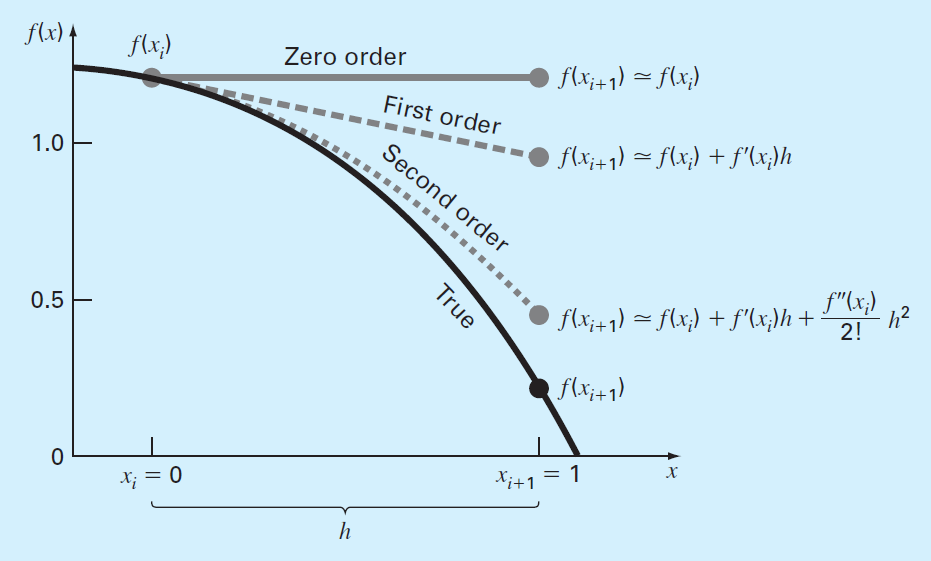
\includegraphics[width=0.8\linewidth]{./images/fig_4_7}
    \caption{The approximation of $f(x)=-0.1x^4 - 0.15x^3 - 0.5x^2 - 0.25x =1.2$ at $x = 1$ by
    zero-order, first-order, and second-order Taylor series expansions.}
\end{figure}
\bigskip




\end{document}
